% Template for ICIP-2015 paper; to be used with:
%          spconf.sty  - ICASSP/ICIP LaTeX style file, and
%          IEEEbib.bst - IEEE bibliography style file.
% --------------------------------------------------------------------------
\documentclass{article}
\usepackage{spconf,amsmath,graphicx}
\usepackage{listings}
\usepackage{float}
\usepackage{pythonhighlight}
% Example definitions.
% --------------------
\def\x{{\mathbf x}}
\def\L{{\cal L}}

% Title.
% ------
\title{Processamento Digital de Imagens - Projeto Individual}
%
% Single address.
% ---------------
\name{Bruna Medeiros da Silva - 16/0048711}
\address{UnB - FGA}
%
% For example:
% ------------
%\address{School\\
%	Department\\
%	Address}
%
% Two addresses (uncomment and modify for two-address case).
% ----------------------------------------------------------
%\twoauthors
%  {A. Author-one, B. Author-two\sthanks{Thanks to XYZ agency for funding.}}
%	{School A-B\\
%	Department A-B\\
%	Address A-B}
%  {C. Author-three, D. Author-four\sthanks{The fourth author performed the work
%	while at ...}}
%	{School C-D\\
%	Department C-D\\
%	Address C-D}
%
\begin{document}
%\ninept
%
\maketitle

%
\section{Questão 1 - Ajuste de Intensidade}
Para a realização do ajuste de intensidade, foi utilizada a técnica de \textbf{equalização de histograma}, que possibilita a aplicação de diversas formas diferentes para equilíbrio entre os pixels, mas também não possui muitos requisitos para funcionar, podendo ser aplicado em diversas imagens e casos diferentes. 

\subsection{Metodologia}
O processo de especificação de histograma pode ser descrito em alguns passos:

\begin{enumerate}
	\item Encontrar o histograma da imagem, que mostra graficamente a a distribuição de níveis de cinza da imagem. Os valores obtidos podem ser chamados de $p_r(r)$;
	
	\item Encontrar os valores $s_k$ da Função de Distribuição Acumulada (CDF - \textit{Cumulative Distribution Function}) da imagem. Para gerar a CDF, foi utilizada a equação \ref{eq:cdf_pr}, que calcula a probabilidade de os pixels possuírem valores menores ou iguais a determinado valor dentro do intervalo de níveis de cinza da imagem. $L$ é igual ao número de níveis de cinza disponíveis ($2^{n_bits}$), $MN$ é a quantidade de pixels que a imagem possui e $k$ é o nível de cinza para o qual estamos fazendo o cálculo e $p_r(j)$ é o valor de $j$ no histograma;
	
	\item Encontrar os valores $z_k$ da CDF da função especificada. Gerar a CDF a partir de uma PDF (\textit{Probability Density Function}) é um processo ainda mais simples, visto que nós já temos a probabilidade de cada valor, precisando apenas somá-los aos anteriores para obter a CDF equivalente (Equação \ref{eq:cdf_pz}). Onde $p_z(j)$ é a probabilidade de um pixel ter o valor $j$. Nesse caso, a PDF padrão utilizada na função implementada foi uma pdf que distribui igualmente os pixels em toda a escala de cinza disponível (geralmente, em \textit{uint8}, se trata de 0 a 255);
	
	\item Fazer a equivalência entre os valores de s para z. Para encontrar o valor $z = G^{-1}(s)$, precisamos encontrar o menor z para o qual $G(z)$ seja o mais próximo possível de $s_k$.
	Fazendo isso para todos os valores de s, teremos o valor equivalente em z para todos os níveis de cinza presentes na imagem;
	
	\item utilizar a nova CDF obtida para gerar uma nova imagem equalizada com os valores dos pixels $s_k$ convertidos para $z_k$.
	
	\item Depois disso, apenas aplicamos essa transformação nos pixels da imagem e, caso necessário, geramos os novos gráficos de histograma, PDF e/ou CDF para efeitos de comparação.
\end{enumerate}

\begin{equation}
\label{eq:cdf_pr}
s_k = \frac{(L - 1)}{MN}\sum_{j = 0}^{k} p_r(j)
\end{equation}

\begin{equation}
\label{eq:cdf_pz}
G(z) = \sum_{j = 0}^{z} p_z(j)
\end{equation}
%\vspace{-pt}

\begin{figure}[H]
	\label{fig: q1_1}
	\begin{minipage}[b]{1.0\linewidth}
		\centering
		\centerline{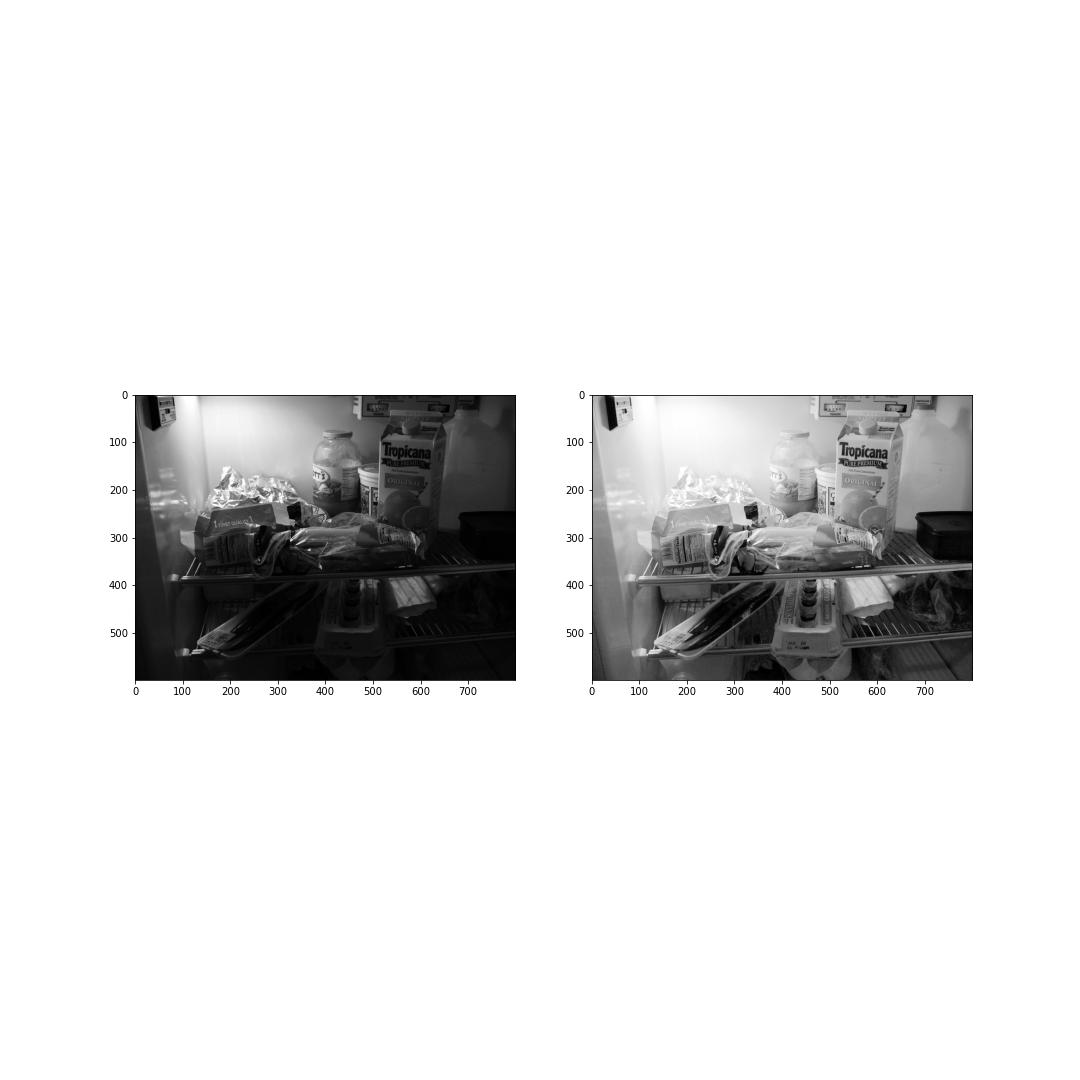
\includegraphics[width=8.5cm]{Figures/result1_1}}
		\centerline{Resultado questão 1 - Imagem 1}\medskip	
	\end{minipage}
\end{figure}

\begin{figure}[H]
	\label{fig: q1_2}
	\begin{minipage}[b]{1.0\linewidth}
		\centering
		\centerline{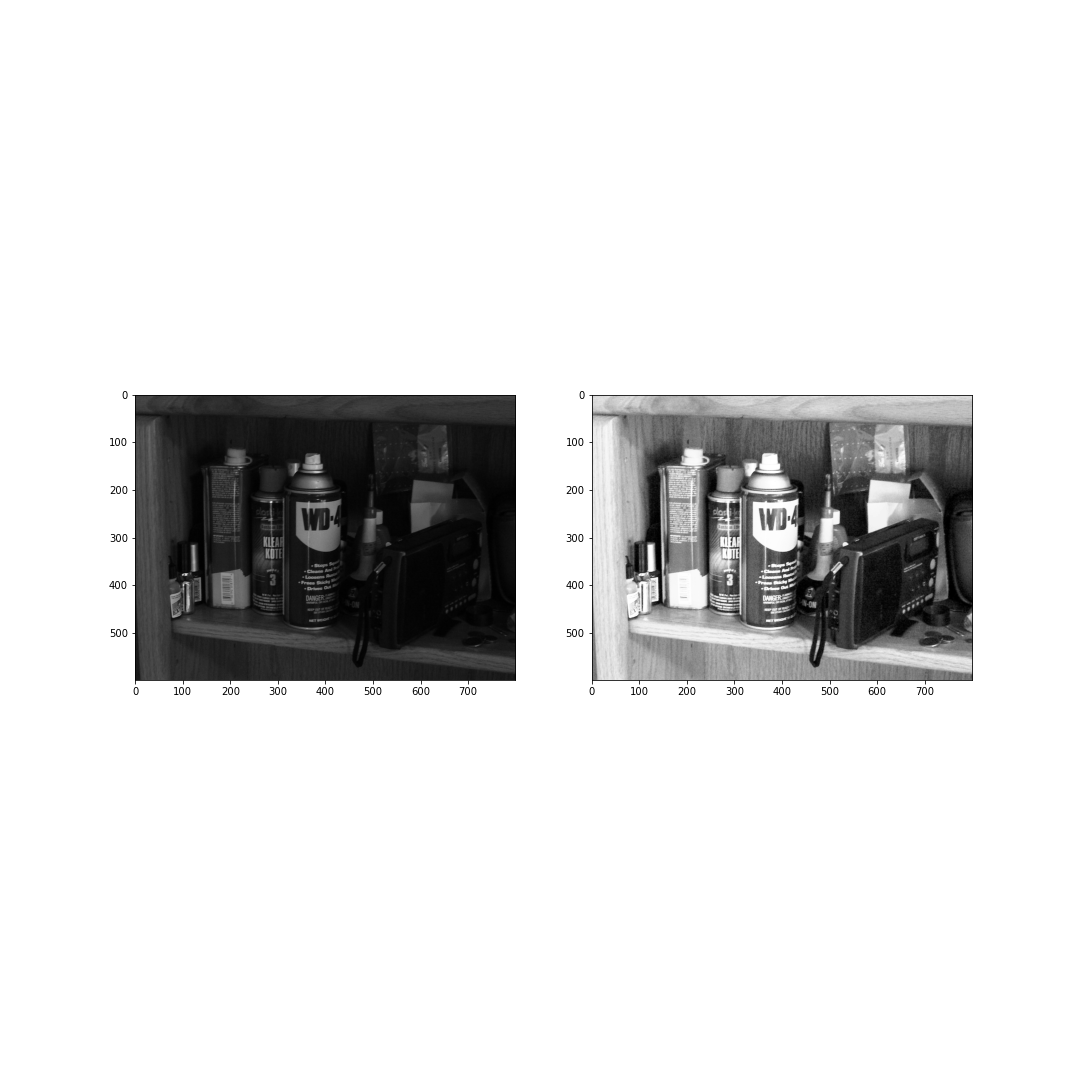
\includegraphics[width=8.5cm]{Figures/result1_2}}
		\centerline{Resultado questão 2 - Imagem 1}\medskip	
	\end{minipage}
\end{figure}

\section{Questão 2 - Realce de Imagem de baixa resolução}
Para a questão 2 foram testados 2 métodos para realce de imagens: aplicação do laplaciano e do filtro butterworth. Isso porque observou-se que o Laplaciano, em muitos casos, gera resultados bem mais significativos na obtenção de realce, resultando em uma imagem visualmente com muito mais nitidez e transmitindo uma impressão de maior qualidade para quem vê.

Em ambas as aplicações, a imagem foi percorrida e modificada por meio de um laço duplo, iterando em cada uma de suas colunas e linhas.

\subsection{Butterworth} 

O filtro butterworth utilizado foi um filtro passa-altas, com o intuito de destacar apenas componentes de alta frequência da imagem (como bordas e detalhes) e depois somá-los à imagem original, gerando uma imagem com detalhes mais destacados. Outra opção também seria utilizar o filtro gaussiano,mas observou-se que os resultados com o mesmo não foram muito significativos, optando-se assim pelo butterworth \ref{eq: butter}.

\begin{align} \label{eq: butter}
     D &= ((u - (P/2))^2 + (v - (Q/2))^2)^{1 / 2} \\
	H[u][v] &= \frac{1}{1 + (D_0/D)^(2n)}
\end{align}

Para obter a imagem final, utilizou-se da fórmula entregue no livro texto da disciplina. Com isso, dentro da função, faz-se necessário que o usuário defina apenas 2 parâmetros: a imagem e o valor $D_0$, que equivale ao raio do filtro a ser aplicado na frequência da imagem. para a transformada para o domínio da frequência, utilizou-se a fft implementada na biblioteca \textit{numpy} do Python.

\begin{figure}[H]
	\label{fig: q2_1_butter}
	\begin{minipage}[b]{1.0\linewidth}
		\centering
		\centerline{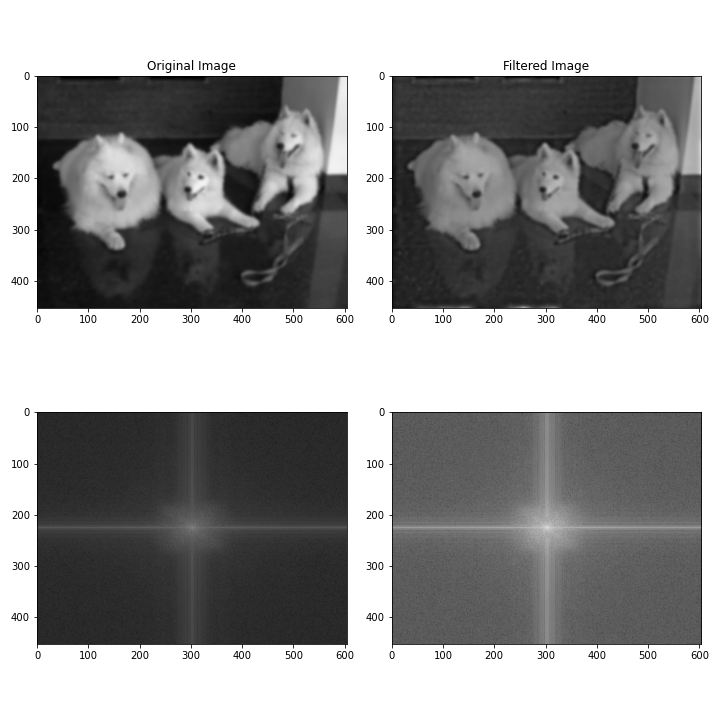
\includegraphics[width=8.5cm]{Figures/result2_1_butter}}
		\centerline{Resultado questão 2 - Imagem 1 com Butterworth}\medskip	
	\end{minipage}
\end{figure}

\begin{figure}[H]
	\label{fig: q2_2_butter}
	\begin{minipage}[b]{1.0\linewidth}
		\centering
		\centerline{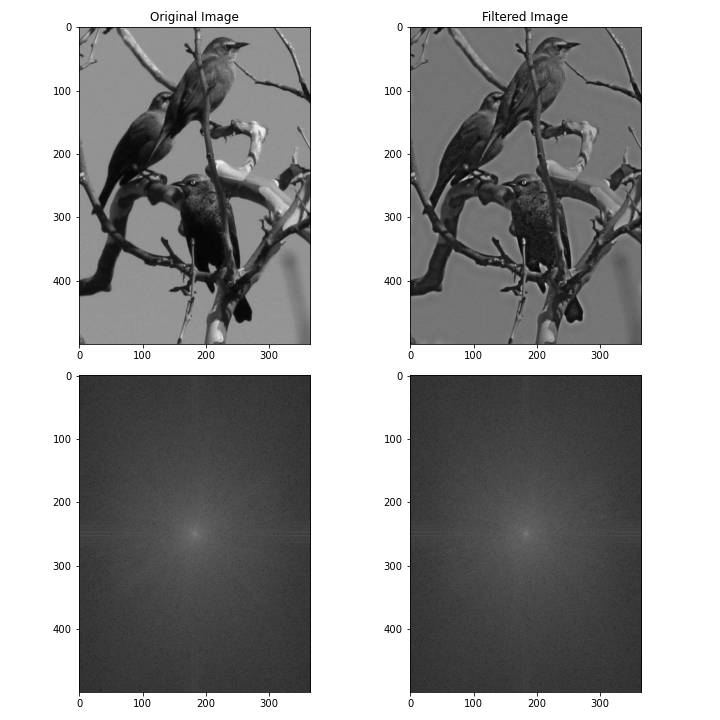
\includegraphics[width=8.5cm]{Figures/result2_2_butter}}
		\centerline{Resultado questão 2 - Imagem 2 com Butterwoth}\medskip	
	\end{minipage}
\end{figure}

\subsection{Laplaciano}
Diferentemente do filtro Butterworth, no Laplaciano o usuário não define os valores do filtro. Todos os valores estão definidos dentro da equação e dependem apenas de valores extraídos de forma subentendida durante o envio da imagem como parâmetro da transformação (como tamanho/\textit{shape} da imagem, por exemplo).

\begin{align}
     D &= ((u - (P/2))^2 + (v - (Q/2))^2)^{1 / 2} \\
	H[u][v] &= - 4 (\pi^2) D^2
\end{align}

\begin{figure}[H]
	\label{fig: q2_1_laplace}
	\begin{minipage}[b]{1.0\linewidth}
		\centering
		\centerline{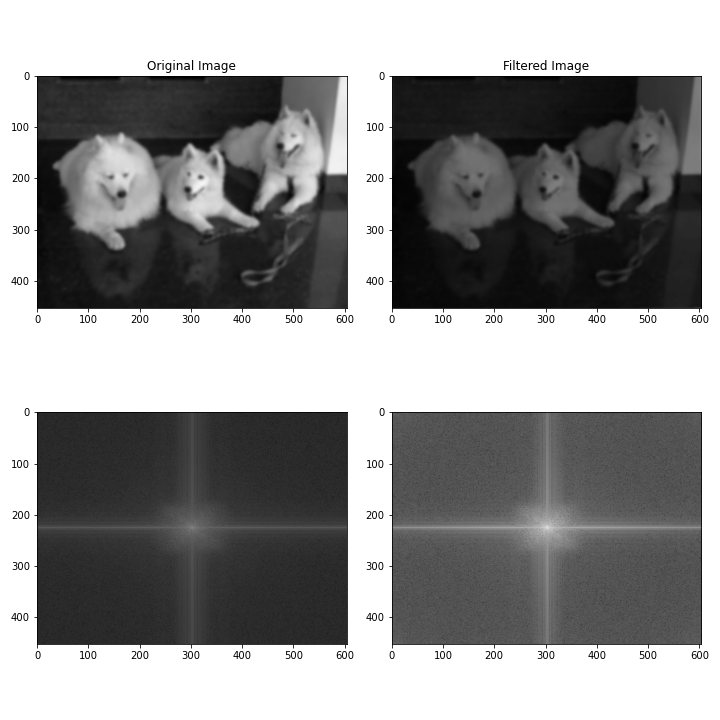
\includegraphics[width=8.5cm]{Figures/result2_1_laplace}}
		\centerline{Resultado questão 2 - Imagem 1 com Laplaciano}\medskip	
	\end{minipage}
\end{figure}

\begin{figure}[H]
	\label{fig: q2_2_laplace}
	\begin{minipage}[b]{1.0\linewidth}
		\centering
		\centerline{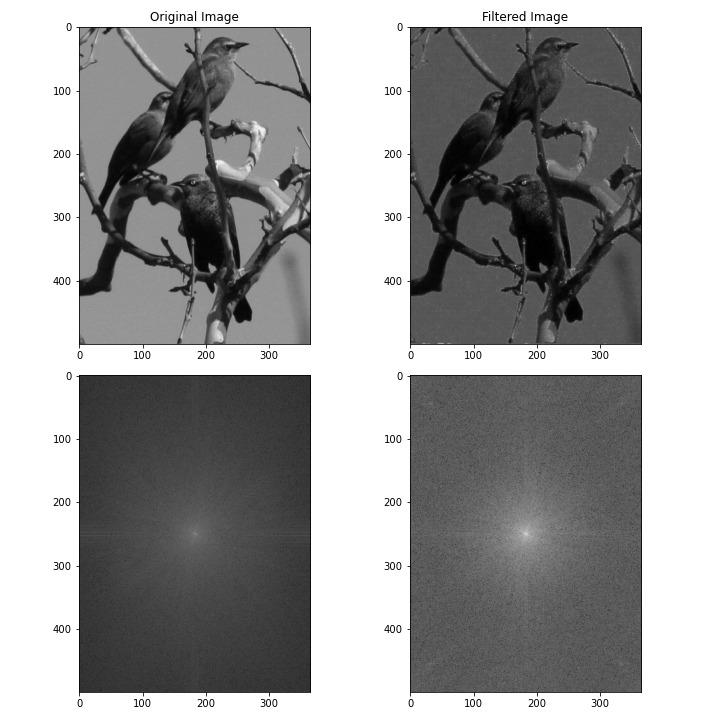
\includegraphics[width=8.5cm]{Figures/result2_2_laplace}}
		\centerline{Resultado questão 2 - Imagem 2 com Laplaciano}\medskip	
	\end{minipage}
\end{figure}

\section{Questão 3 - Filtragem de ruído}
Para a filtragem de alguns ruídos, foi utilizado um \textbf{filtro de média retangular}. Com essa aplicação, o usuário tem a liberdade de definir o tamanho da janela utilizada para fazer a média, o que definirá o quanto a imagem será suavizada. O uso de janela excessivamente grandes para o tamanho e conteúdo da imagem fazem com que a imagem passe a ficar "borrada" e comece a perder informações e detalhes. Esse efeito de "borramento" possui uma relação diretamente proporcional ao tamanho da janela utilizada na média.

Para evitar extrapolar as fronteiras da imagem durante o processo, realiza-se a filtragem apenas em pixels nos quais pode-se colocar toda a janela sem que nenhum de seus pixels fique "fora" das bordas da imagem original.

\begin{figure}[H]
	\label{fig: q3_1}
	\begin{minipage}[b]{1.0\linewidth}
		\centering
		\centerline{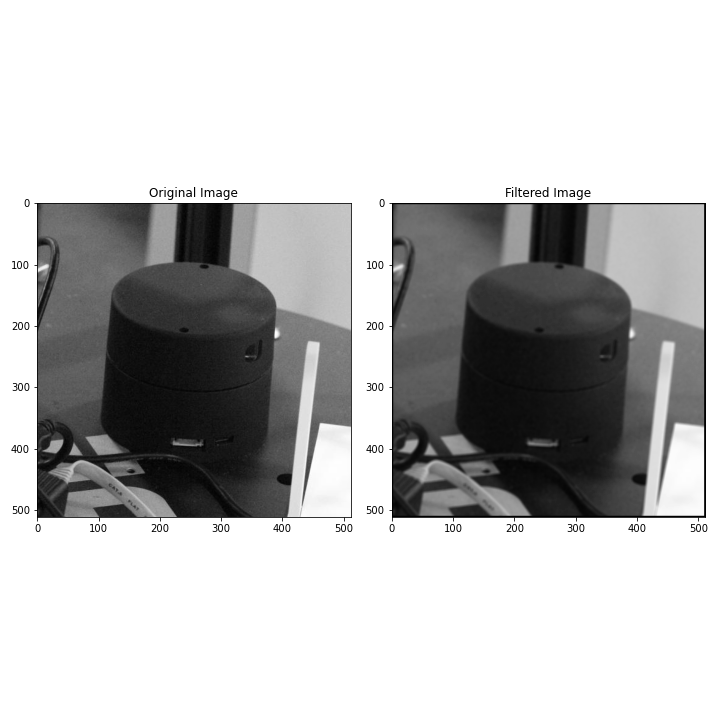
\includegraphics[width=8.5cm]{Figures/results3_1}}
		\centerline{Resultado questão 3 - Imagem 1}\medskip	
	\end{minipage}
\end{figure}

\begin{figure}[H]
	\label{fig: q3_2}
	\begin{minipage}[b]{1.0\linewidth}
		\centering
		\centerline{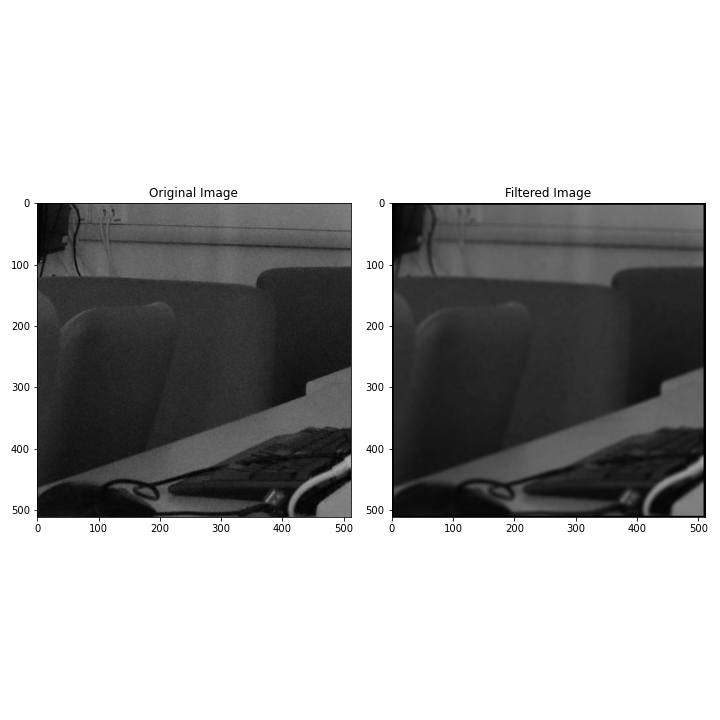
\includegraphics[width=8.5cm]{Figures/results3_2}}
		\centerline{Resultado questão 3 - Imagem 2}\medskip	
	\end{minipage}
\end{figure}

\section{Questão 4 - Granulometria}
Para separar determinados componentes de uma imagem e possibilitar a remoção de alguns outros, de acordo com seu tamanho e formato, pode-se realizar a técnica de \textbf{segmentação por textura}, aplicando assim o estudo da granulometria dentro do tratamento de imagens.

Dentro do projeto, foram utilizadas imagens com "bolhas" e componentes circulares de diversos tamanhos. Para a identificação desses componentes, realiza-se a diferença entre a soma de todos os pixels da imagem após o processo de abertura com diferentes tamanhos de kernel. Realizando essa comparação e plotando seus resultados, torna-se possível identificar o tamanho dessas componentes, que equivale aos picos do gráfico. 

A técnica foi utilizada para separar círculos de diferentes tamanhos, podendo gerar imagens diferentes com cada um deles, se necessário.

É importante ressaltar que antes da aplicação também é possível e recomendado que seja realizado o processo de suavização da imagem, que consiste em realizar a abertura e o fechamento da imagem, respectivamente.

Essa técnica é estabelecida para casos em que esses componentes são mais claros que os valores de fundo. Na tentativa de adaptá-los, é possível passar parâmetros para a função de suavização que realizam o processo de forma inversa (primeiro o fechamento e depois a abertura da imagem). 

\begin{figure}[H]
	\label{fig: q4_1}
	\begin{minipage}[b]{1.0\linewidth}
		\centering
		\centerline{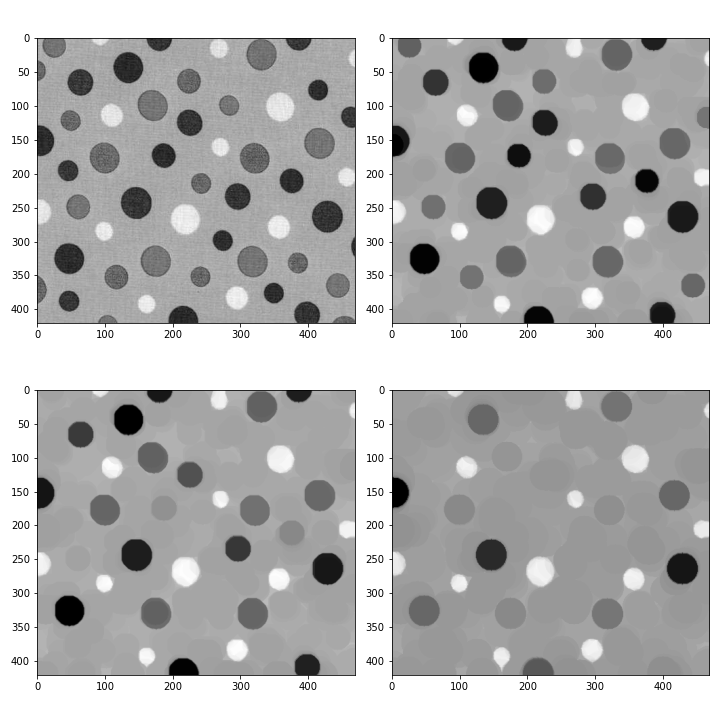
\includegraphics[width=8.5cm]{Figures/result4_1}}
		\centerline{Resultado questão 4 - Imagem 1}\medskip	
	\end{minipage}
\end{figure}

\begin{figure}[H]
	\label{fig: q4_1_graph}
	\begin{minipage}[b]{1.0\linewidth}
		\centering
		\centerline{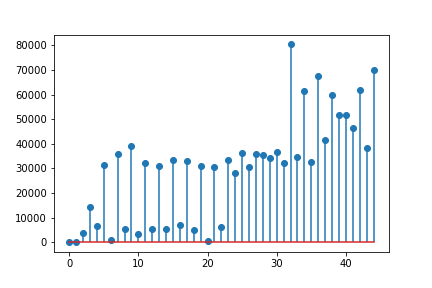
\includegraphics[width=8.5cm]{Figures/result4_1_graph}}
		\centerline{Resultado questão 4 - Gráfico da Imagem 1}\medskip	
	\end{minipage}
\end{figure}

\begin{figure}[H]
	\label{fig: q4_2}
	\begin{minipage}[b]{1.0\linewidth}
		\centering
		\centerline{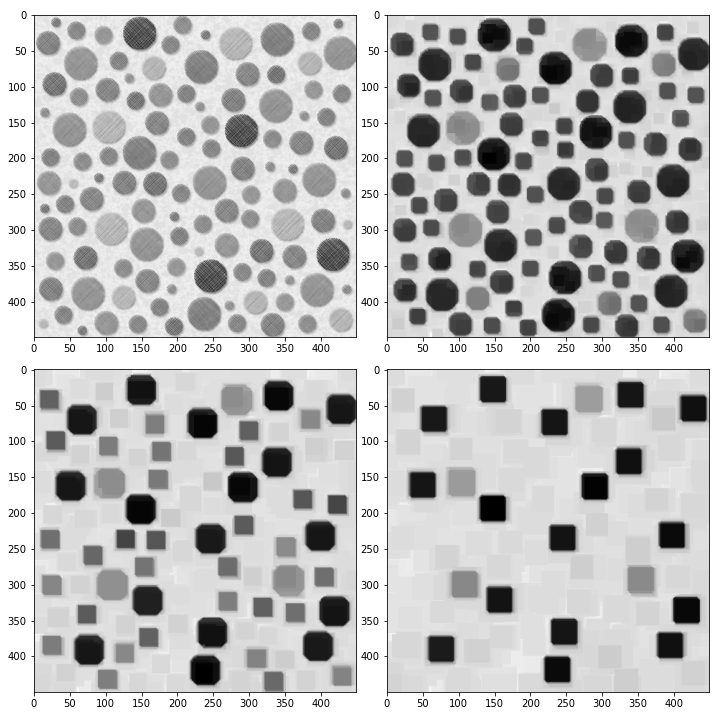
\includegraphics[width=8.5cm]{Figures/result4_2}}
		\centerline{Resultado questão 4 - Imagem 2}\medskip	
	\end{minipage}
\end{figure}

\begin{figure}[H]
	\label{fig: q4_2_graph}
	\begin{minipage}[b]{1.0\linewidth}
		\centering
		\centerline{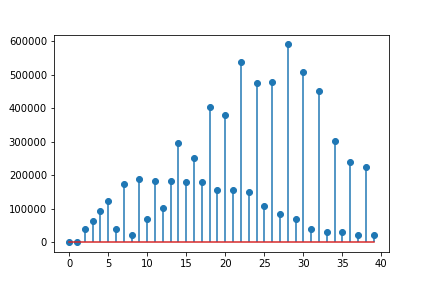
\includegraphics[width=8.5cm]{Figures/result4_2_graph}}
		\centerline{Resultado questão 4 - Gráfico da Imagem 2}\medskip	
	\end{minipage}
\end{figure}

\textbf{Obs.: Os códigos-fonte estão em anexo, todos compactados em um arquivo .zip.}

\end{document}
